\documentclass[a4paper,12pt]{article} 
\usepackage[T1,T2A]{fontenc} 
\usepackage[utf8]{inputenc}
\usepackage[russian]{babel}
\usepackage{amssymb,amsfonts,amsmath,mathtext,cite,enumerate,float}
\usepackage[hidelinks]{hyperref}
\usepackage{graphicx}
\usepackage{adjustbox}
\usepackage {indentfirst}
\usepackage{amsmath}
\usepackage{indentfirst}
\usepackage{bbm}
%\usepackage[linesnumbered,boxed]{algorithm2e}

\usepackage{geometry} % Меняем поля страницы
\geometry{left=2cm}% левое поле
\geometry{right=2cm}% правое поле
\geometry{top=1cm}% верхнее поле
\geometry{bottom=2cm}% нижнее поле

\newcommand{\argmin}{\operatornamewithlimits{argmin}}
%\newcommand{\min}{\operatornamewithlimits{min}}
%для русского псевдокода
%\SetKwInput{KwData}{Входные данные}
%\SetKwInput{KwResult}{Результат}
%\SetKwInput{KwIn}{Входные данные}
%\SetKwInput{KwOut}{Выходные данные}
%\SetKwIF{If}{ElseIf}{Else}{если}{тогда}{иначе\ если}{иначе}{конец\ условия}
%\SetKwFor{While}{до\ тех\ пор,\ пока}{выполнять}{конец\ цикла}
%\SetKw{KwTo}{от}
%\SetKw{KwRet}{возвратить}
%\SetKw{Return}{возвратить}
%\SetKwBlock{Begin}{начало\ блока}{конец\ блока}
%\SetKwSwitch{Switch}{Case}{Other}{Проверить\ значение}{и\ выполнить}{вариант}{в\ противном\ случае}{конец\ варианта}{конец\ проверки\ значений}
%\SetKwFor{For}{цикл}{выполнять}{конец\ цикла}
%\SetKwFor{ForEach}{для\ каждого}{выполнять}{конец\ цикла}
%\SetKwRepeat{Repeat}{повторять}{до\ тех\ пор,\ пока}
%\SetAlgorithmName{Алгоритм}{алгоритм}{Список алгоритмов}

\usepackage{algorithm}
\usepackage{algpseudocode}

\renewcommand{\listalgorithmname}{Список алгоритмов}
\floatname{algorithm}{Алгоритм}

\algrenewcommand\algorithmicwhile{\textbf{До тех пока}}
\algrenewcommand\algorithmicdo{\textbf{выполнять}}
\algrenewcommand\algorithmicrepeat{\textbf{Повторять}}
\algrenewcommand\algorithmicuntil{\textbf{Пока}}
\algrenewcommand\algorithmicend{\textbf{Конец}}
\algrenewcommand\algorithmicif{\textbf{Если}}
\algrenewcommand\algorithmicelse{\textbf{иначе}}
\algrenewcommand\algorithmicthen{\textbf{тогда}}
\algrenewcommand\algorithmicfor{\textbf{Цикл}}
\algrenewcommand\algorithmicforall{\textbf{Выполнить для всех}}
\algrenewcommand\algorithmicfunction{\textbf{Функция}}
\algrenewcommand\algorithmicprocedure{\textbf{Процедура}}
\algrenewcommand\algorithmicloop{\textbf{Зациклить}}
\algrenewcommand\algorithmicrequire{\textbf{Вход:}}
\algrenewcommand\algorithmicensure{\textbf{Выход:}}
\algrenewcommand\algorithmicreturn{\textbf{Выход:}}
\algrenewtext{EndWhile}{\textbf{Конец цикла}}
\algrenewtext{EndLoop}{\textbf{Конец зацикливания}}
\algrenewtext{EndFor}{\textbf{Конец цикла}}
\algrenewtext{EndFunction}{\textbf{Конец функции}}
\algrenewtext{EndProcedure}{\textbf{Конец процедуры}}
\algrenewtext{EndIf}{\textbf{Конец условия}}
\algrenewtext{EndFor}{\textbf{Конец цикла}}
\algrenewtext{BeginAlgorithm}{\textbf{Начало алгоритма}}
\algrenewtext{EndAlgorithm}{\textbf{Конец алгоритма}}
\algrenewtext{BeginBlock}{\textbf{Начало блока. }}
\algrenewtext{EndBlock}{\textbf{Конец блока}}
\algrenewtext{ElsIf}{\textbf{иначе если }}




\begin{document}
\begin{titlepage}
\begin{center}

    \bigskip
    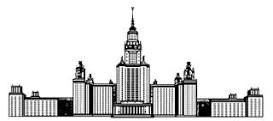
\includegraphics[width=50mm]{titul_cartoon}

    \bigskip
    Московский государственный университет имени М.\,В.~Ломоносова
    Факультет Вычислительной математики и кибернетики\\
    Кафедра Математических методов прогнозирования\\[30mm]

    \textsf{\large
      ВЫПУСКНАЯ КВАЛИФИКАЦИОННАЯ РАБОТА \\[10mm]
      \textbf{
        Построение ансамбля алгоритмов рекомендаций
      }
    }\\[30mm]

    \begin{flushright}
      \parbox{0.5\textwidth}{
        \raggedleft
        \textbf{Выполнил:}\\
        студент 417 группы\\
        Кудрявцев Георгий Алексеевич\\[5mm]
        \textbf{Научный руководитель:}\\
        д.ф-м.н., профессор\\
        Дьяконов Александр Геннадьевич
      }
    \end{flushright}

    \vspace{\fill}
    Москва, 2015
\end{center}
\end{titlepage}
\thispagestyle{empty} % не нумеровать первую страницу
\newpage

\tableofcontents % сгенерировать оглавление
\newpage
\section{Введение}
%Что такое и зачем рекомендательные системы.
%Что такое Коллаборативная фильтрация
%Вида методов колллаборативной фильтрации
%Что такое явный и неявный отклик.
%Наша задача + объяснение ее актуальности

С ростом популярности электронной коммерции, возникла задача помощи пользователям в поиске товаров, которые им понравятся. Одними из инструментов, используемые для решения этой проблемы, являются рекомендательные системы. 

Коллаборативная фильтрация является одним из методов построения рекомендательных систем. Она использует известные оценки или предпочтения пользователей для построения рекомендации пользователям, чьи оценки и предпочтения неизвестны. Идея данного метода состоит в предположении того, что пользователи, имеющие похожие предпочтения в прошлом, будут иметь похожие предпочтения в будущем.



Существует три различных подхода в коллаборативной фильтрации.

Первый подход называется Memory-based. Его идея заключается в вычислении сходства между пользователями или предметами. Соответственно, похожие предметы или пользователи должны иметь похожие оценки или предпочтения.

Второй подход называется Model-based. Его идея заключается в создание моделей при помощи интеллектуального анализа данных и машинного обучения. Модель обучается на реальных данных, например, на истории покупок интернет-магазина, а далее выдает рекомендации для пользователей, чьи предпочтения неизвестны. 

Третий подход -- Hybrid. Его идея заключается в использовании первого и второго подхода, компенсируя недостатки обоих. 


В данной работе будет рассматриваться второй подход.

Также следует упомянуть о таком важном понятии как обратная связь(feedback). Обратной связью некоторого пользователя на предмет называют некоторое событие, по которому можно судить о предпочтении автора. 
Например, это может быть оценка фильма по десятибалльной шкале. Либо клик на описание товара в интернет-магазине.

В коллаборативаной фильтрации выделяют два типа обратной связи: с явным откликом(explicit feedback) и неявным откликом(implicit feedback).

 В первом случае пользователь осознано оценивает предмет и производит соответствующий отклик. Например, пользователь оценивает работу интернет-магазина по пятибалльной шкале.

Неявный отклик  означает лишь, что между пользователем и предметом произошло взаимодействие. Например, покупатель зашел на страницу с описанием товара, либо несколько раз посмотрел  видеоролик. Как видно, из этого отклика нельзя выяснить имеется ли у пользователя положительное или отрицательное предпочтение к предмету, и есть ли оно вообще.

В данной работе будет рассмотрен случай, в котором набор данных состоит только из неявного отклика, причем он будет в бинарном виде, то есть '1' - будет означать, что пользователь имел взаимодействие с предметом и '0', если такого взаимодействия не было.  Такая ситуация возможна в некоторых случаях. Например, дружба между пользователями в социальной сети или история встреч на сайте знакомств. Далее будем считать, что неявный отклик показывает положительное предпочтение пользователя к предмету.


В качестве моделей будет рассмотрен класс факторизационных методов. Их основная идея лежит в представлении предпочтения пользователя к предмету  в виде скалярного произведения их латентных векторов\cite{matrixfactorization}.  Данные методы хорошо себя показали в известном конкурсе Netflix Prize\cite{netflix}.

Также в решении победителей не малую роль сыграл ансамбль алгоритмов. Поэтому в данной работе было  решено исследовать, как можно улучшить качество современных факторизационных методов в задаче ранжирования при помощи  построения ансамблей. 

\section{Цель работы}
Целью работы является изучение и сравнение существующий факторизационных методов ранжирования, а также создание новых, более эффективных при помощи построения ансамблей. 


Данная работа  разделена на несколько частей.
\begin{enumerate}
\item Ввод необходимых понятий и обозначений.
\item Обзор современных методов ранжирования.
\item Построение различных ансамблей методов ранжирования.
\item Тестирование и сравнение методов и ансамблей на реальных данных.
\end{enumerate}


\section{Обозначения}

Набор данных R представлен в виде матрицы  размером $|U| \times |I|$, где $U$ - множество пользователей, и $I$ - множество предметов. В дальнейшем обозначим $M = |U| $ и $N = |I|$

Если между пользователем $u$ и предметов $i$ произошел неявный отклик, то $R_{ui}=1$. В противном случае $R_{ui} = 0$. Будем считать, что предмет $i$ релевантен пользователю $u$, если $R_{ui}$


Обозначим за $rank(u, i)$ номер позиции предмета i в упорядоченном списке, который был получен при помощи метода ранжирования, для пользователя $u$.   

Введем функцию $rel(u, k)$ такую что, $rel(u, k)$ = 1, если предмет, стоящий на $k$ позиции в упорядоченном списке предметов для пользователя $u$, релевантен. В противном случае $rel(u, k)$ = 0.  


Пусть  

$P$ - множество профилей пользователей, 

$Q$ - множество профилей предметов,

$P_u$ - профиль(латентный вектор) пользователя $u$ и

$Q_i$ - профиль(латентный вектор) предмета $i$.

Прогноз $f_{ui}$ предпочтения пользователя $u$ предмета $i$ будет представлен в виде скалярного произведения латентных векторов $P_u$ и $Q_i$, т.е. $f_{ui} = \langle P_u, Q_i \rangle$

Также в дальнейшем будет часто использоваться сигмоида. Обозначим ее за $\sigma(x) = \frac{1}{1 + e^{-x}}$. 
%\section{Постановка задачи}
%
%Дана матрица описаний транзакций R. По ней нужно построить метод ранжирования, который будет для каждого пользователя $u$ выдавать список предметов в порядке релевантности. Будем считать, что предмет $i$ релевантен пользователю $u$, если $R_{ui} =1$.

\section{Критерии качества}
В задаче ранжирования не существует однозначно правильного функционала качества. Поэтому было решено использовать сразу несколько.

\subsection{$P@n$}
	Определим эту метрику для одного пользователя.
	\begin{equation*}
		P@n(u) = \frac{1}{N}\sum_{k = 1}^n rel(u, k)
	\end{equation*}
	
	Теперь для всех пользователей.
	\begin{equation*}
		P@n = \frac{1}{M}\sum_{u = 1}^M P@n(u)
	\end{equation*}
	$P@n$ показывает среднюю долю релевантных объектов по всем пользователям.  Недостатком этой метрики является то, что она не учитывает порядок предметов. Например,  если пользователь получил только один релевантный предмет, то для этой метрики не важно, был ли он в начале списка или в конце. 
\subsection{$1call@n$}
	Определим эту метрику для одного пользователя.
	\begin{equation*}
		1call@n(u) = [\sum_{k = 1}^n rel(u, k) > 0]
	\end{equation*}
	
	Теперь для всех пользователей.
	\begin{equation*}
		P@n = \frac{1}{M}\sum_{u = 1}^M 1call@n(u)
	\end{equation*}
	$1call@n$ показывает долю запросов по всем пользователям, у которых был хотя бы один релевантный предмет. Метрика не учитывает  ни порядок, ни количество релевантных предметов. 
\subsection{$MRR$}
	MRR -- Mean Reciprocal Rank
	
	Пусть $firstrank(u)$  - номер позиции первого релевантного предмета в ранжированном списке для пользователя $u$. Номер позиции в списке начинается с 1.
	\begin{equation*}
		MRR = \frac{1}{M}\sum^{M}_{u=1}\frac{1}{firstrank(u)}	
	\end{equation*}
	
	Эта метрика используется, если рекомендательной системе важнее подать пользователю один релевантый предмет в начало списка. 

	 
\subsection{$NDCG@n$}
	NDCG -- Normalized Discounted Cumulative Gain
	
	\begin{equation*}
	\begin{split}
	 & G(u, k) = 2^{rel(u, k)} - 1 \\
	 & D(k) = \frac{1}{log_2(k + 1)} \\
	 & DCG@n(u) = \sum_{k=1}^n G(u, k) D(k) \\
	 & NDCG@n(u) = \frac{DCG@n(u)}{max DCG@n}
	\end{split}			
	\end{equation*}
	
	Эта метрика является популярной в информационном поиске. Она учитывает и порядок, и количество релевантных предметов. Также большим плюсом является то, что $NDCG$ работает в случае различных уровней релевантностей.
	
\subsection{$MAP$}
	MAP -- 	Mean Average Precision
	
	
	\begin{equation*}
	\begin{split}
	 & AP@n(u) = \frac{1}{n}\sum_{k=1}^n rel(u, k) P@k(u)  \\
	 & MAP@n = \frac{1}{M}\sum_{k=1}^M AP@n(u) \\
	\end{split}			
	\end{equation*}
	
	Аналогично предыдущей метрике, $MAP$ является достаточно популярной, учитывает и порядок, и количество релевантных предметов.
	
	
%\subsection{$AUC$}

\section{Существующие методы}
В ходе работы были рассмотрены факторизационные методы ранжирования. Их основная идея заключается в представлении пользователей и предметов в виде векторов латентных векторов $P_u$ и $Q_i$. Величина $f_{ui} = \langle P_u, Q_i\rangle$  показывает заинтересованность пользователя $u$ в предмете  $i$. Соответственно, по величине $f_{ui}$ можно ранжировать предметы для конкретного пользователя.
	
Далее приведен список факторизационных методов с их кратким описанием.  
\begin{enumerate}
\item \textbf{CLiMF} --
  Факторизационный метод, который оптимизирует сглаженную версию метрики MRR.\cite{climf}
  	
\item \textbf{MPR\_MF} -- 
  Факторизационный метод, который оптимизирует AUC.\cite{bprmp}
  
\item \textbf{TFMAP} --
   Факторизационный метод, который оптимизирует сглаженную метрику MAP.\cite{tfmap}

\item \textbf{iMF} --
	Факторизационный метод, который оптимизирует взвешенную квадратичную ошибку.\cite{imf} 

\item \textbf{PopRec} --
    Простой метод, который ранжирует предметы по убыванию количества пользователей, для которых данный предмет является релевантным. В результате метод выдает для каждого пользователя один  и тот же ответ.
\end{enumerate}

\subsection{CLiMF}
Данный метод использует в качестве функционала качества MRR. Заметим, что MRR можно переписать в другом виде.
\begin{equation*}
 MRR =\frac{1}{M}\sum_{u=1}^M \sum_{i=1}^N \frac{R_{ui}}{rank(u,i)}\prod_{k=1}^N(1 - R_{uk}[rank(u,k) < rank(u, i)])
\end{equation*}
 Но  MRR не является гладкой функцией, поэтому авторы метода решили оптимизировать сглаженную версию этой метрики. В качестве регуляризатора был взят L2-регуляризатор. В итоге получаем следующий функционал качества.

\begin{equation*}
	F(P, Q) = \sum_{u=1}^M \sum_{i=1}^N [R_{ui}(\ln(\sigma(f_{ui})) + \sum_{k=1}^N \ln(1 - R_{uk}\sigma(f_{uk} - f_{ui})))] - \frac{\lambda}{2}({||U||}^2 + {||V||}^2 ) 
	\end{equation*}	

Далее этот функционал оптимизируется при помощи стохастического градиентного спуска.

\begin{algorithm}[h]
\caption{обучение метода CLiMF}
\begin{algorithmic}[1]
\Require {набор данных R, параметр регуляризации $\lambda$, скорость обучение $\gamma$, 
максимальное число итерации maxiter}
\Ensure {обученные латентные векторы P, Q}
\For{i = 1 .. M}
\State $N_u = \{i | R_{ui} > 0, 1 \leq i \leq N\}$
\EndFor

инициализируем $U^{(0)}$ и $V^{(0)}$ случайными значениями. t = 0.
\Repeat {} 
\For {$u = 1 .. M$}
		\State $P_u^{(t+1)} = P_u^{(t)} + \gamma \frac{\partial F}{\partial P_u^{(t)}}$
			\For {$i \in N_u$}
				\State 	$Q_i^{(t+1)} = Q_i^{(t)} + \gamma \frac{\partial F}{\partial 	  																						Q_i^{(t)}}$		
			\EndFor	
	\EndFor 
\Until{$t \leq itermax$}

\end{algorithmic}
\label{alg:climf}
\end{algorithm}
\newpage
\subsection{BRP\_MF}  	

Авторы данного метода применили байесовкий подход к решению задачи ранжирования. Для каждого пользователя $u$  предметы были разбиты на 3 класса: релевантные и нерелевантные предметы, а также предметы с неизвестной релевантностью. Собственно, для последнего класса и нужно было строить ранжирование. 



Пусть $\theta$ - параметр метода. В нашем случае это $P$ и $Q$.  $I_u^+$ -- множество релевантных предметов пользователя u. $I_u^-$ -- множество нерелевантных предметов пользователя u.  $>_u$ - это ранжированный список предметов для пользователя u. Требуется максимизировать вероятность $p(\theta|>_u)$.
\begin{equation*}
\begin{split}
	& p(\theta| >_u) \propto p(>_u| \theta)p(\theta) \\
	& p(>_u| \theta) = \prod_{i, j: \ i \in I_u^+, j \in I_u^-}p(i >_u j| \theta)\\
	& p(\theta) \sim N(0, \lambda I) \\
	& p(i >_u j| \theta) = \sigma(f_{ui} - f_{uj}) 
\end{split}
\end{equation*}

В итоге имеем следующий функционал качества. 
\begin{equation*}
F(P, Q) = \ln(p(\theta| >_u)) = \ln(p(>_u|\theta)p(\theta)) = \sum_{u,i,j: u \in U\ i \in I_u^+\ j \in I_u^-}\ln(\sigma(f_{ui} - f_{uj})) - \lambda {||\theta||} ^ 2
\end{equation*}


Нормальное априорное распределение задает L2-регуляризацию, а сигмоида позволяет легко высчитывать производные для данного функционала. Авторами  было показано, что данный алгоритм оптимизирует AUC.

\begin{algorithm}[h]
\caption{обучение метода BRP\_MP}
\begin{algorithmic}[1]
\Require {набор данных R, параметр регуляризации $\lambda$, скорость обучение $\gamma$, 
максимальное число итерации maxiter}
\Ensure {обученные латентные векторы P, Q}
\State {Инициализируем $\theta$ случайными значениями, t = 0}
\Repeat {} 
	\State {берем случайную тройку $(u, i,j)$, где $u \in U, i \in I_u^+, j \in I_u^-$} 
	\State {$\theta = \theta + \alpha \big( \frac{1}{1 + e ^{(f_{ui} - f_{uj})}}  
	\frac{\partial}{\partial \theta} (f_{ui} - f_{uj}) + \lambda \theta \big)$} 
	\State {t = t + 1}
\Until{$t \leq itermax$}

\end{algorithmic}
\label{alg:climf}
\end{algorithm}

\newpage
\subsection{iMF}
За основу iMF был взят оригинальный SVD, функционал качества которого выглядит следующим образом.

\begin{equation*}
F(P, Q) = \sum_{R_{ui} - \textnormal{известно}} (R_{ui} - f_{ui})^2 + \lambda ({||P||} ^ 2 + {||Q||}^2)
\end{equation*}

Недостаток SVD заключается в том, что он показывает плохое качество ранжирования в поставленной задаче.
Чтобы преодолеть данную проблему, авторы метода поменяли функционал качества на следующий.

\begin{equation*}
\begin{split}
& F(P, Q) = \sum_{u, i} c_{ui}(g_{ui} - f_{ui})^2 + \lambda ({||P||} ^ 2 + {||Q||}^2) \\
& g_{ui} =  \begin{cases} 
   0  &\mbox{если } R_{ui} = 0 \\ 
   1 & \mbox{если } R_{ui} > 0 
\end{cases} \\
& c_{ui} = 1 + \alpha R_{ui}
\end{split}
\end{equation*}

Переменная $g_{ui}$ отвечает за неявный отклик между пользователем $u$ и предметом $i$. Т.е. iMF пытается определить не уровень предпочтения пользователя, а неявный отклик. Хотя в нашем случае это одно и тоже. 

Переменная $c_{ui}$ является весом каждого квадратного слагаемого. Чем больше предпочтение, тем больше вес. 

Метод обучается при помощи ALS\cite{matrixfactorization}. 

Пусть Q -- матрица профилей предметов размера $N \times K$, где K - размерность латентного вектора. Каждая $i$-ая  строка равна латентному вектору предмета $i$.  $C^u$ -- диагональная матрица размера $N \times N$, в которой $C_{ii}^u = c_{ui}$. $S_u$ -- вектор размера $N$, в котором $S_{ui} = R_{ui}$. Тогда латентный вектор пользователя $u$ обновляется по следующей формуле.

\begin{equation*}
	P_u = (Q^TC^uQ + \lambda I) ^ {-1}Q^TC^uS_u
\end{equation*} 

Заметим, что $(Q^TC^uQ + \lambda I) = Q^TQ + Q^T(C^u - I)Q $. Матрицу $Q^TQ$ можно вычислить один раз перед обновлением всех латентных векторов пользователй, а в матрице $C^u - I$ количество ненулевых элементов равно числу взаимодействий пользователя $u$ с предметами.

Для латентных векторов рассуждения аналогичны.

\begin{algorithm}[h]
\caption{обучение метода iMF}
\begin{algorithmic}[1]
\Require {набор данных R, параметр регуляризации $\lambda$, скорость обучение $\gamma$, 
максимальное число итерации maxiter}
\Ensure {обученные латентные векторы P, Q}
\State {Инициализируем $P$ и $Q$ случайными значениями, t = 0}
\Repeat {} 
	\State {вычислить матрицу $Q^TQ$} 
	\For {$u = 1 .. M$}
	\State{обновить $P_u$}
	\EndFor
	\State {вычислить матрицу $P^TP$}
	\For {$i = 1 .. N$}
	\State{обновить $Q_i$}
	\EndFor
\Until{$t \leq itermax$}

\end{algorithmic}
\label{alg:climf}
\end{algorithm}


%
%Переменная g_{ui} отвечает за неявный отклик. Будем делать прогноз не на $R_{ui}$, а на $g_{ui}$. Хотя в нашем случае это одно  и то же.  Также заметим, что намного 

\subsection{TFMAP}
Данный метод использует в качестве функционала качества MAP. Заметим, что MAP можно переписать в следующем виде. 
\begin{equation*}
 MAP = \frac{1}{M}\sum_{u=1}^M\frac{\sum_{i=1}^N \frac{R_{ui}}{rank(u, i)} \sum_{j=1}^N R_{uj} 
 [rank(u,j) \leq rank(u, i)]}{\sum_{i=1}^N R_{ui}} 
\end{equation*} 
 
 Далее проводятся рассуждения аналогичные CLiMF. Метрика TFMAP  не является гладкой, следовательно, будем оптимизировать приближенную гладкую версию это метрики. Также добавим L2-регуляризатор.
 
 В итоге получаем  следующую формулу.
 \begin{equation*}
 \begin{split}
 & F(P, Q) = \sum_{u=1}^M \frac{1}{\sum_{i=1}^N R_{ui}} \sum_{i=1}^N R_{ui} \sigma(f_{ij}) \times \sum_{j=1}^N R_{mj} \sigma(f_{uj} - f_{ui}) - \frac{1}{2}\lambda({||P||}^2 + {||Q||}^2)
 \end{split}
 \end{equation*}

Далее возникает проблема подсчета частной производной по $Q_i$. Она вычисляется при помощи следующей формулы. 

\begin{equation*}
 \frac{\partial F}{\partial Q_i} = \sum_{u=1}^M\frac{R_{ui} P_u}{\sum_{i=1}^N R_{ui}}\sum_{j=1}^N \Big(\sigma^{\prime}( f_{ui})\sigma(f_{uj} - f_{ui}) + (\sigma(f_{uj}) - \sigma(f_{ui}))\sigma^{\prime}(f_{uj} - f_{ui}) \Big )  R_{ui} - \lambda Q_i
\end{equation*}

Сложность вычисления этого выражения -- $O(KN|R|)$, где $K$ - размерность латентных векторов, $|R|$ -  количество взаимодействий пользователей с предметами. На практике подсчет такой производной несет большие вычислительные затраты. Для ускорения вычисления выражения авторы заменили $\sum_{i=1}^N$ на $\sum_{i \in B_{u}}$, где $B_{u}$ - множество предметов специального вида. Далее приведен алгоритм построения этого множества.

\begin{algorithm}[h]
\caption{построение множества $B_{u}$}
\begin{algorithmic}[1]
\Require {$Q_i$ и $f_{ui}$ для всех $i$,  размер выборки $n$, $P_u$}
\Ensure {$B_u$}
\State {$B_u = \emptyset$}
\State $B_u = B_u \cup \{i | R_{ui} = 1 \}$
\State $n_u = |B_u|$
\State $p = \min_{i \in B_u} f_{ui}$
\State $S  = \{i |R_{ui} = 0 \} \cap \{i| f_{ui} > p \}$
\State Случайно выбираем подмножество $L \subset S$ размера n.
\State Отсортируем предметы $i \in L$ по убыванию $f_{ui}$
\State Выбираем первые $n_u$ предметов из полученного списка. Обозначим это множество предметов за $B^{-}$
\State $B_u = B_u \cup B^{-}$  
\end{algorithmic}
\label{alg:setB}
\end{algorithm}

Метод обучается при помощи стохастического градиентного спуска.


\section{Эксперименты}

\subsection{Наборы данных}
В исследовании были использованы 4 разных набора данных.

\begin{itemize}
\item \textbf{Epinion} - социальная сеть, в которой публикуются покупательские отзывы и рецензии на товары и услуги. Каждый участник  решает кому он "доверяет". Следовательно, если пользователь $u$ "доверяет" пользователю $i$, то $R_{ui} = 1$

\item \textbf{Slashdot} - сайт, который предоставляет различные новости в сфере IT. Пользователи сами публикуют новости, в то время как другие пользователи их оценивают и обсуждают. Также данный сайт предоставляет возможность пользователям объявлять друг друга "врагом" или "другом".  $R_{ui}$ = 1, если пользователь $u$ является "другом" или "врагом" пользователя $i$.

\item \textbf{MovieLens} - сайт, в котором пользователи рекомендуют различные фильмы друг другу. Movielens предоставляет возможность ставить оценки фильмам. $R_{ui}$ = 1, если пользователь $u$ поставил оценки фильму $i$. В данной работе использованы два различных набора данных MovieLens: в первом 100000 оценок, во втором 1000000.

\end{itemize}

Перед тем как использовать наборы данных в экспериментах, из них были удалены пользователи, которые взаимодействовали с менее  25 предметами. Это было сделано для преодоления проблемы холодного старта, которым страдают факторизационные методы. 

Далее приведены статистические характеристики каждого набора данных после предобработки. 



\begin{table}[H]
\caption{\label{tab:canonsummary}Статистические характеристики}
\begin{center}
\begin{tabular}{|c|c c c c|}
\hline
Набор данных  & Epinion & Slashdot & MovieLens100k & MovieLens1m\\
\hline
Число ненулевых элементов & 326114 & 573578 & 96963  & 989202 \\
Число пользователей & 4405 & 6992 & 806 & 5549\\
Число предметов & 34777 & 63730 & 1682 & 3702\\
Плотность матрицы & 0.21\% & 0.13\% & 7.15 \% & 4.81 \% \\
Среднее число предметов у пользователя & 51  & 50 & 81 & 106\\
Максимальное число пользователей & 1801 & 2508 & 737 & 2314\\
у одного предмета.  & & & &\\
\hline
\end{tabular}
\end{center}
\end{table} 

\subsection{Сравнение методов}
 Сравним качество работы методов ранжирования друг с другом. Для этого проведем следующий эксперимент.
 
 Разобьем набор данных на тренировочную и тестовую выборку случайным образом. В тренировочной выборке у каждого пользователя будет trainK предметов. Остальные предметы лежат в тестовой выборке. Алгоритмы обучаются на тренировочной выборке, а качество работы измеряется на тестовой выборке. Далее такой эксперимент повторяется maxiter раз. Конечным результатом является средняя величина качества работы по метрикам и алгоритмам. 
 
Параметры методов были настроены при помощи кросс-валидации на наборе данных Epinion. 
 
На таблицах \ref{tab:modsepinion}, \ref{tab:modsslashdot}, \ref{tab:modsmovk} и \ref{tab:movm} показано качество работы алгоритмов на различных данных и параметрах эксперимента.

\begin{table}[H]
\caption{Набор данных Epinion}
\label{tab:modsepinion}
%\begin{center}
\resizebox{0.8\textwidth}{!}{\begin{minipage}{\textwidth}
\begin{tabular}{|c|c|c|c|c|c|c|c|c|c|c|}
\hline
& \multicolumn{5}{|c|}{trainK = 5, maxiter = 5} & \multicolumn{5}{|c|}{trainK = 10, maxiter = 5}\\
\hline
  & PopRec & CLiMF & BRP\_MF & iMF & TFMAP & PopRec & CLiMF & BRP\_MF & iMF & TFMAP  \\
\hline
P@5 & \textbf{0.1987}& 0.1962 &	0.1960 & 0.1876 & 0.1807 & 0.1837  & 0.1844 & 0.1846 & \textbf{0.2613} &	0.1808 \\
\hline
1call@5 & \textbf{0.5632} & 0.5448 & 0.5450 & 0.5509 & 0.5448 & 0.5189 & 0.5293 & 0.5241 &	\textbf{0.6383} & 0.5212\\
\hline
NDCG@5 & \textbf{0.2222} & 0.2205 & 0.2205 & 0.1980 & 0.2104 & 0.2061 & 0.2064 & 0.1909 &	\textbf{0.2725} &0.2041\\
\hline
MAP@5 & 0.3813 & 0.3769 & 0.3774 & 0.3356 & \textbf{0.3873} & 0.3568 & 0.3572 & 0.3120 &	\textbf{0.4121} & 0.3597\\
\hline
MRR & \textbf{0.4387} & 0.4368 & 0.4383 & 0.3818 & 0.4306 & 0.4113 & 0.4112 & 0.3480 & \textbf{0.4609} &	0.4114\\
\hline
AUC  & 0.8307 & 0.7512 & \textbf{0.8347} & 0.6915 & 0.6407 & 0.8558 & 0.8143 & \textbf{0.8591} &	0.8105 & 0.7310\\
\hline
\end{tabular}
\end{minipage}}
%\end{center}
\end{table} 


\begin{table}[H]
\caption{Набор данных Slashdot}
\label{tab:modsslashdot}
%\begin{center}
\resizebox{0.8\textwidth}{!}{\begin{minipage}{\textwidth}
\begin{tabular}{|c|c|c|c|c|c|c|c|c|c|c|}
\hline
& \multicolumn{5}{|c|}{trainK = 5, maxiter = 5} & \multicolumn{5}{|c|}{trainK = 10, maxiter = 5}\\
\hline
  & PopRec & CLiMF & BRP\_MF & iMF & TFMAP & PopRec & CLiMF & BRP\_MF & iMF & TFMAP  \\
\hline
P@5 & 0.1225 & \textbf{0.1227} & 0.1210 & 0.1049 & 0.1153 &  0.1119 & 0.1118 & 0.1128 & \textbf{0.1358} & 0.1128 \\
\hline
1call@5 & \textbf{0.3765} & 0.3774 & 0.3761 & 0.3419 & 0.3592 & 0.3528 & 0.3528 & 0.3531 &	\textbf{0.3928} & 0.3544\\
\hline
NDCG@5 & \textbf{0.1319} & 0.1316 & 0.1309 & 0.1097 & 0.1244 & 0.1210 & 0.1210 & 0.1207 &	\textbf{0.1424} & 0.1215\\
\hline
MAP@5 & 0.2295 & 0.2289 & 	\textbf{0.2297}	& 0.1949 &	0.2194 &  0.2146 & 	0.2147 & 0.2110 &  \textbf{0.2374} &	0.2148\\
\hline
MRR & \textbf{0.2765} & 0.2755 &  0.2761 &  0.2343 &	0.2567 & 0.2602 & 0.2598  & 0.2558 & \textbf{0.2794} & 0.259429\\
\hline
AUC & 0.7770 &	0.6897 & \textbf{0.7850} & 0.5908 & 0.5973 &  0.8127	& 0.7582 & \textbf{0.8182} &	0.6925 & 0.6662\\
\hline
\end{tabular}
\end{minipage}}
%\end{center}
\end{table} 


\begin{table}[H]
\caption{Набор данных MobieLens 100k}
\label{tab:modsmovk}
%\begin{center}
\resizebox{0.8\textwidth}{!}{\begin{minipage}{\textwidth}
\begin{tabular}{|c|c|c|c|c|c|c|c|c|c|c|}
\hline
& \multicolumn{5}{|c|}{trainK = 5, maxiter = 5} & \multicolumn{5}{|c|}{trainK = 10, maxiter = 5}\\
\hline
  & PopRec & CLiMF & BRP\_MF & iMF & TFMAP & PopRec & CLiMF & BRP\_MF & iMF & TFMAP  \\
\hline
P@5 & \textbf{0.5309} & 0.5131 & 0.5303 & 0.4625 & 0.2624 &  0.4841 & 0.4821 &  0.4738 & \textbf{0.5307} & 0.4738 \\
\hline
1call@5 & \textbf{0.9431} & 0.9334 &	0.9374 & 0.8970 & 0.7461 & 0.9146 &	0.9141 & 0.9074 & \textbf{0.9292} &	0.8937\\
\hline
NDCG@5 & \textbf{0.5341} & 0.5171 &	0.5319 & 0.4756 & 0.3055 &  0.4934 & 0.4958 & 0.4725 &  \textbf{0.5369} &	0.4802\\
\hline
MAP@5 & \textbf{0.6703} & 0.6512 & 0.6636 & 0.6341 & 0.5452 & 0.6492 & 0.6568 & 0.6117 & \textbf{0.6741} &	0.6212\\
\hline
MRR & \textbf{0.7045} & 0.6970 &	0.7019 & 0.6818 & 0.5931 &  0.6885 & 0.6984 & 0.6474 &	\textbf{0.7139} & 0.6660\\
\hline
AUC & 0.8274 & 0.7572 &	\textbf{0.8288} & 0.6785 & 0.6366 &  0.8530 & 0.8405 & \textbf{0.8531} &	0.8285 & 0.7634\\
\hline
\end{tabular}
\end{minipage}}
%\end{center}
\end{table} 


\begin{table}[H]
\caption{Набор данных MobieLens 1m}
\label{tab:movm}
%\begin{center}
\resizebox{0.8\textwidth}{!}{\begin{minipage}{\textwidth}
\begin{tabular}{|c|c|c|c|c|c|c|c|c|c|c|}
\hline
& \multicolumn{5}{|c|}{trainK = 5, maxiter = 5} & \multicolumn{5}{|c|}{trainK = 10, maxiter = 5}\\
\hline
  & PopRec & CLiMF & BRP\_MF & iMF & TFMAP & PopRec & CLiMF & BRP\_MF & iMF & TFMAP  \\
\hline
P@5 & 0.4805 &	\textbf{0.4835} & 0.4797 & 0.4739 & 0.4138 &  0.4903 & 0.4903 &	0.4835 & \textbf{0.5739} & 0.4906\\
\hline
1call@5 & 0.8805 & 0.8704 & \textbf{0.8826} & 0.8707	& 0.8538 &  0.8610 & 0.8610 & 0.8479 & \textbf{0.9302} &	0.8587\\
\hline
NDCG@5 & \textbf{0.4935} & 0.4952 & 0.4923 &	0.4850 & 0.4515 & 0.5011 & 0.5011 &	0.4918 & \textbf{0.5838} & 0.5014\\
\hline
MAP@5 &0.6489 &	\textbf{0.6534} & 0.6484 & 0.6285 & 	0.6626 & 0.6557 & 0.6557 & 0.6151 &  \textbf{0.7088} & 0.6594 \\
\hline
MRR & \textbf{0.6941} & 0.6916 &	0.6930 & 0.6728 & 0.7019 & 0.6903 &	0.6903 & 0.6597 & \textbf{0.7530} & 0.6897\\
\hline
AUC & \textbf{0.8503} & 0.8286 &	0.8488 & 0.7185 & 0.7476 & \textbf{0.8561} &	0.8514 & 0.8556 & 0.8279 & 0.8043\\
\hline
\end{tabular}
\end{minipage}}
%\end{center}
\end{table} 

Видно, что качество работы методов сильно зависит от проводимого эксперимента. 

При trainK = 5 в среднем лучше работает PopRec. Во многом высокое качество работы PopRec связано с тем, что во всех представленных наборах данных существует большое количество популярных предметов, которые есть почти у каждого пользователя. Например, очередной блокбастер или  популярный блог. С данной проблемой сталкивались авторы других статей \cite{climf, reasonbadwork}.
 
 CLiMF, BRP\_MF и TFMAP всегда имеют качество работы близкое к PopRec. Но в отличие от PopRec, факторизационные методы имеют разные прогнозы предпочтения для разных пользователей.  
 
 В результатах экспериментов также не  было замечено какой-либо хорошей работы CLiMF и TFMAP на метриках MRR и MAP@n соответственно. Причем не один из данных методов не имел самое высокое качество по своему функционалу. 
 
 BRP\_MF почти всегда имеет самый высокий AUC. Но по второму эксперименту видно,что такой функционал абсолютно не подходит. iMF имеет самое высокое качество на втором эксперименте по всем метрикам, кроме AUC. 
 
 Далее в данной работе будут проведены эксперименты по улучшению качества работы путем ансамблирования 4 факторизационных методов.

\subsection{Составление линейного  ансамбля}


Пусть имеется множество базовых алгоритмов $b_i(x)$. Необходимо подобрать такие веса $\alpha_i$, чтобы линейная комбинация алгоритмов $\hat{b}(x) = \sum_i \alpha_i b_i(x)$ показывала лучший результат по какому-нибудь заданному функционалу. 

В нашем случае $b_i$ - методы ранжирования описанные ранее. Каждый метод возвращает ранжированный список предметов, который неудобно использовать в задаче ансамблирования. Удобнее использовать величину $f_{ui}$, которую можно интерпретировать как меру предпочтения. Обозначим  за $f_{ui}^m$ значение $f_{ui}$ $m$-ого базового метода.

Заметим, что для алгоритмов ранжирования  важно не само значение $f_{ui}$, а их порядок друг относительно друг. Поэтому диапазон значений этой величины у каждого алгоритма разный и зависит от функционала качества и регуляризатора. Поэтому, чтобы линейный комбинации были корректны,  необходимо нормировать значения $f_{ui}$ для каждого пользователя $u$. В результате $0 \leq f_{ui} \leq 1$. Далее будем считать, что все $f_{ui}$ нормированы.

  Рассмотрим несколько способов создание ансамблей:
 
\begin{itemize}
\item Простое голосование. 
\item Взвешенное голосование при помощи линейной регрессии.
\item Оптимальное взвешенное голосование
\end{itemize}
%Каждый факторизационный метод возвращает для пользователя $u$ множество значений $f_ui$ для всех $i$, которые можно интерпретировать как меру предпочтения пользователя $u$ предмета $i$.
Для экспериментов над ансаблями наборы данных были разбиты на 3 выборки: тренировочную, тестовую и валидационную. На тренировочной обучаются факторизационые методы, на валидационной настраиваются веса, а на тестовой вычисляется качество работы ансамбля. Размер тренировочной и валидационной выборки для каждого пользователя одинаков и равен traink и validk соответственно. В тестовой выборке лежат все остальные предметы.

\subsubsection*{Простое голосование}
Один из простейших методов, который представляет из себя линейную комбинацию базовых методов с равными весами.
\begin{equation*}
 	\hat{b}(x)= \frac{1}{T}\sum_{m = 1} ^ T b_m(x)
\end{equation*}

В случае ранжирования данная выражение будет выглядеть следующим образом.

\begin{equation*}
	\hat{f}_{ui} = \frac{1}{T}\sum_{m = 1} ^ T f_{ui}^m
\end{equation*}
\subsubsection*{Взвешенное голосование при помощи линейной регрессии}

Линейная регрессия была одним из самых простых способов ансамблирования, которые были реализованы победителями конкурса Netflix.  Основная  проблема линейной регрессии и всех остальных методов агрегирования из этого конкурса в том, что они оптимизируют совершенно другой функционал. А именно RMSE. Но с другой стороны iMF тоже хорошо справляется с  задачей хоть и не оптимизирует на прямую метрики ранжирования.

Для каждого пользователя  выберем 5 предметов из валидационной выборки. Они все релевантные. Далее случайным образом выберем 25 предметов, которые не лежат ни в валидационной, ни в тренировочной выборке, и объявим из нерелевантными. В итоге из этих предметов строим матрицу признаков $X$ и целевой вектор $y$. 

\begin{table}[H]
\label{tab:schemetable}
\begin{center}
\begin{tabular}{|c|c|c|c|c|}
\hline
 \multicolumn{4}{|c|}{X} & \multicolumn{1}{|c|}{y}\\
\hline
  $f_{ui_1} ^ {m_1}$& $f_{ui_1} ^ {m_2}$ & $f_{ui_1} ^ {m_3}$& $f_{ui_1} ^ {m_4}$& $R_{ui_1}$ \\
\hline
$f_{ui_2} ^ {m_1}$& $f_{ui_2} ^ {m_2}$ & $f_{ui_2} ^ {m_3}$& $f_{ui_2} ^ {m_4}$& $R_{ui_2}$ \\
\hline
$f_{ui_3} ^ {m_1}$& $f_{ui_3} ^ {m_2}$ & $f_{ui_3} ^ {m_3}$& $f_{ui_3} ^ {m_4}$& $R_{ui_3}$ \\
\hline
$f_{ui_4} ^ {m_1}$& $f_{ui_4} ^ {m_2}$ & $f_{ui_4} ^ {m_3}$& $f_{ui_4} ^ {m_4}$& $R_{ui_2}$ \\
\hline
... & ... & ... &  ... & ... \\
\end{tabular}
\end{center}
\caption{Схематичное изображение признаковой матрицы}
\end{table} 

Далее обучаем  линейную регрессию на матрице признаков X и на целевом векторе y. 

\subsubsection*{Оптимальное взвешенное голосование} 
      Рассмотрим линейную комбинацию двух алгоритмов ранжирования  в следующем виде:
\begin{equation*}
	\hat{f}_{ui} = \alpha f_{ui}^{m_1} + (1 - \alpha) f_{ui} ^ {m_2} \textrm{\ , где $0 \leq \alpha \leq 1$} 
\end{equation*}


	Заметим, что все метрики ранжирования меняются только при изменении порядка предметов в ранжированном списке, а не от самого изменения $f_{ui}$. Поэтому число различных значений метрики не может быть больше конечного числа. На рис.\ref{pic:latexpic} видно, что изменения порядка происходит в точках пересечения линий. Их  не более чем $O(|U||I|^2)$. 

\begin{figure}[h]
\center{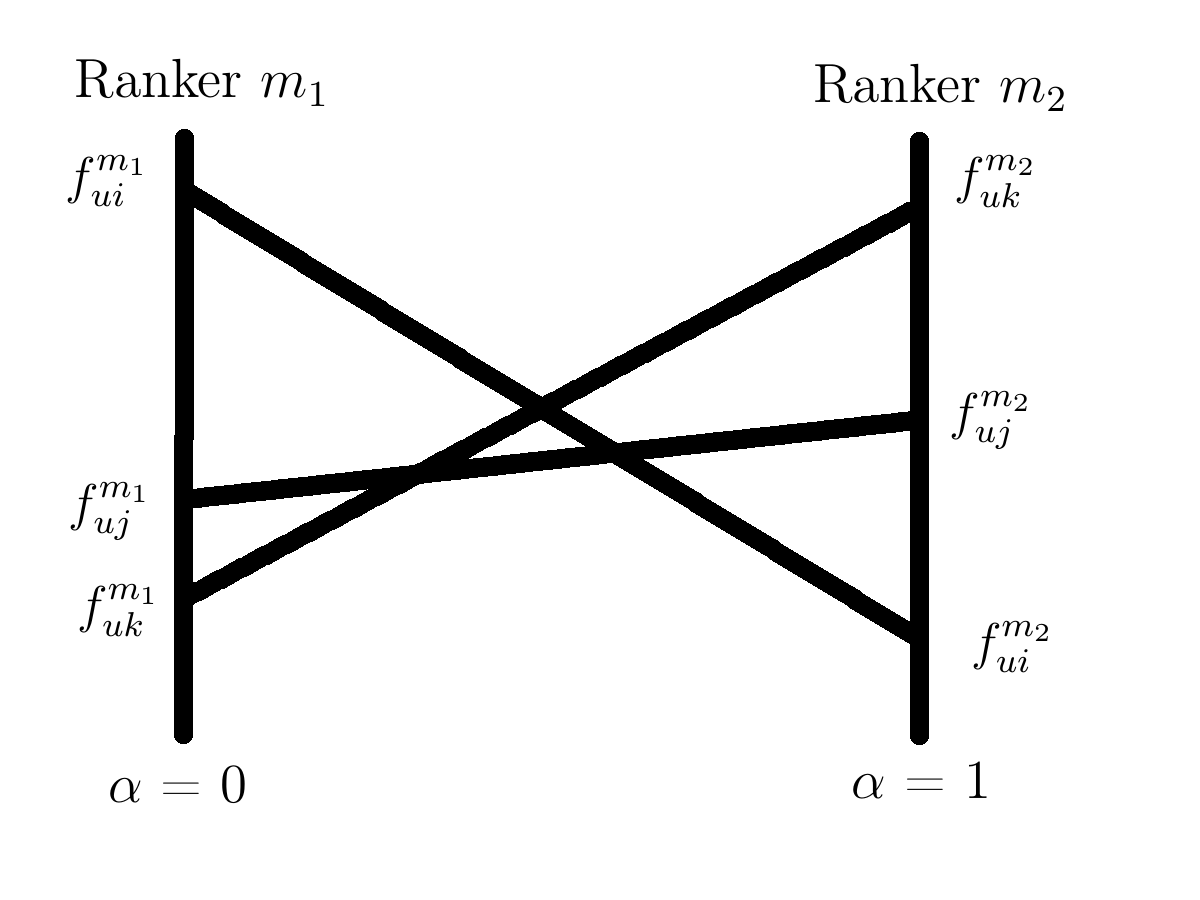
\includegraphics[width=0.4\linewidth]{latexpic}}
\caption{Две вертикальные линии обозначают размер величины f. Чем выше точка, тем больше величина. Невертикальные линии обозначают линейные комбинации величин f. Если $\alpha$ = 0, то линейная комбинация учитывает только Ranker $m_1$, если $\alpha = 1$, то  линейная комбинация учитывает только Ranker $m_2$}
\label{pic:latexpic}
\end{figure}
	
	Идея метода состоит в вычислении качества ансамбля при различных $\alpha$ на валидационной выборке в поисках оптимального параметра. Теоретически  можно перебрать все значения $\alpha$, при которых значение метрики различны. Но количество различных точек $\alpha$ слишком велико, поэтому было решено брать только малое подмножество точек. Далее было замечено, если брать $\alpha$ равномерно от 0 до 1, то результат получается такой же. В экспериментах был использован последний вариант.
	
	Обозначим за $b(x) = (b_i, b_j)$ ансамбль двух алгоритмов при помощи оптимального взвешенного голосования. 
	Обобщим оптимальное взвешенное голосование для 4 методов двумя способами:
	\begin{itemize}
	\item при помощи бустинга. $(((b_1, b_2), b_3), b_4)$
	\item при помощи построения дерева. $((b_1,b_2), (b_3, b_4))$
	\end{itemize}
	
\subsection*{Сравнение работы ансамблей}
Введем несколько обозначений.
\begin{itemize}
\item 
BSM(best single method) - лучшее значение метрики достигаемое одиночным методом.
\item 
SV(Simple Vote)  - простое голосование.
\item 
RV(Regression Vote) - взвешенное голосование при помощи линейной регрессии.
\item 
OVB(Optimal Vote Boosting) - оптимальное взвешенное голосование при помощи бустинга.
\item 
OVT(Optimal Vote Tree) - оптимальное взвешенное голосование при помощи построения дерева.
\end{itemize}




\begin{table}[H]
\caption{Набор данных Epinion}
\label{tab:movm}
%\begin{center}
%\resizebox{0.8\textwidth}{!}{\begin{minipage}{\textwidth}
\begin{tabular}{|c|c|c|c|c|c|c|c|c|c|c|}
\hline
& \multicolumn{5}{|c|}{trainK = 5, validk=5, maxiter = 5} & \multicolumn{5}{|c|}{trainK = 10, validk = 5, maxiter = 5}\\
\hline
  & BSM  & SV &  RV & OVB & OVT &BSM  & SV & RV & OVB & OVT \\
\hline
P@5 & 0.1811 & 0.1986 & 0.2033 & \textbf{0.2108} & 0.2095 & 0.2364 & 0.2120& 0.1935& \textbf{0.2438} & 0.2387 \\
\hline
1call@5 & 0.5334  & 0.5622 &0.5707 & \textbf{0.5852} & 0.5847 & 0.6004 & 0.5651&0.5243 & \textbf{0.6190}& 0.6177\\
\hline
NDCG@5 & 0.2028 & 0.2190 & \textbf{0.2230} & 0.2305 & 0.2291 & 0.2456&0.2271 & 0.2060 &\textbf{0.2564} & 0.2529\\
\hline
MAP@5 & 0.3590 & 0.3734 & 0.3784 & \textbf{0.3892}& 0.3872 & 0.3775& 0.3670& 0.3339 &0.3995 & 0.\textbf{4011}\\
\hline
\end{tabular}
%\end{minipage}}
%\end{center}
\end{table} 




\begin{table}[H]
\caption{Набор данных Slashdot}
\label{tab:movm}
%\begin{center}
%\resizebox{0.8\textwidth}{!}{\begin{minipage}{\textwidth}
\begin{tabular}{|c|c|c|c|c|c|c|c|c|c|c|}
\hline
& \multicolumn{5}{|c|}{trainK = 5, validk=5, maxiter = 5} & \multicolumn{5}{|c|}{trainK = 10, validk = 5, maxiter = 5}\\
\hline
  & BSM  & SV &  RV & OVB & OVT &BSM  & SV & RV & OVB & OVT \\
\hline
P@5 &  0.1098 &0.1137 &\textbf{0.1155} & 0.1121 & 0.1127& 0.1272 &0.1137 & 0.1111 &\textbf{0.1333} & 0.1322 \\
\hline
1call@5 &0.3507 & 0.3631& \textbf{0.3729} & 0.3560 & 0.3646 & 0.3796 & 0.3565&0.3760  & 0.4017 &\textbf{0.4071} \\
\hline
NDCG@5 & 0.1192&0.1214 & \textbf{0.1225}& 0.1209 & 0.1212& 0.1340 & 0.1175&0.1250  &\textbf{0.1407} &0.1397 \\
\hline
MAP@5 & 0.2134&0.2143 & \textbf{0.2177} & 0.2147 &0.2166 & 0.2277 & 0.2073 &0.2207&  0.2410& \textbf{0.2419}\\
\hline
\end{tabular}
%\end{minipage}}
%\end{center}
\end{table}



\begin{table}[H]
\caption{Набор данных MovieLens 100k}
\label{tab:movm}
%\begin{center}
%\resizebox{0.8\textwidth}{!}{\begin{minipage}{\textwidth}
\begin{tabular}{|c|c|c|c|c|c|c|c|c|c|c|}
\hline
& \multicolumn{5}{|c|}{trainK = 5, validk=5, maxiter = 5} & \multicolumn{5}{|c|}{trainK = 10, validk = 5, maxiter = 5}\\
\hline
  & BSM  & SV &  RV & OVB & OVT &BSM  & SV & RV & OVB & OVT \\
\hline
P@5 & 0.5142 &0.5243 &0.5124 &\textbf{0.5321} &0.5296 &0.4930 & 0.5298 & \textbf{0.5622} &0.5513 & 0.5573 \\
\hline
1call@5 & 0.9317 & 0.9272& 0.9280 &\textbf{0.9372} &0.9347 & 0.9143& 0.9346& \textbf{0.9346}& 0.9230& 0.9230\\
\hline
NDCG@5 &0.5202 & 0.5392&0.5118 & \textbf{0.5455} & 0.5416&0.5116 & 0.5424 & 0.5727 &0.5647 & \textbf{0.5754}\\
\hline
MAP@5 & 0.6616 & 0.6842 &0.6435 & \textbf{0.6918} & 0.6868 & 0.6708&0.6907 & 0.7060 &0.6979 & \textbf{0.7133}\\
\hline
\end{tabular}
%\end{minipage}}
%\end{center}
\end{table}

%prec@5	0.490819	0.493052	0.487593	0.482630	0.551365	0.557320	0.560050	0.558809
%1recal@5	0.914392	0.914392	0.897022	0.908189	0.923077	0.923077	0.923077	0.925558
%NDCG@5	0.511642	0.508992	0.495114	0.466087	0.564753	0.575404	0.577618	0.576932
%MAP@5	0.670818	0.664066	0.633221	0.578200	0.697991	0.713327	0.714513	0.714859

\begin{table}[H]
\caption{Набор данных MovieLens 1m}
\label{tab:movm}
%\begin{center}
%\resizebox{0.8\textwidth}{!}{\begin{minipage}{\textwidth}
\begin{tabular}{|c|c|c|c|c|c|c|c|c|c|c|}
\hline
& \multicolumn{5}{|c|}{trainK = 5, validk=5, maxiter = 5} & \multicolumn{5}{|c|}{trainK = 10, validk = 5, maxiter = 5}\\
\hline
  & BSM  & SV &  RV & OVB & OVT &BSM  & SV & RV & OVB & OVT \\
\hline
P@5 & 0.4700 & 0.4957 &0.4947& \textbf{0.5104} &0.5028 & 0.5484& 0.5312& 0.4926&0.5709 & \textbf{0.5772}  \\
\hline
1call@5 & 0.8587 &0.8812 & 0.8835  &0.8942 &\textbf{0.8990}  & 0.9131& 0.8835& 0.8574& 0.9201&\textbf{0.9225} \\
\hline
NDCG@5 & 0.4832 & 0.5099& 0.5101&\textbf{0.5268} & 0.5183 & 0.5603 &0.5344 & 0.4990&0.5847 &\textbf{0.5909} \\
\hline
MAP@5 & 0.6442 & 0.6606& 0.6568& \textbf{0.6728}& 0.6684 & 0.6922& 0.6633& 0.6410& 0.7136&\textbf{0.7187} \\
\hline
\end{tabular}
%\end{minipage}}
%\end{center}
\end{table}

\subsection*{Другие эксперименты}
\subsubsection*{Сравнение методов}
\begin{table}[H]
\caption{Набор данных MovieLens 100k}
\label{tab:movm}
%\begin{center}
\resizebox{0.8\textwidth}{!}{\begin{minipage}{\textwidth}
\begin{tabular}{|c|c|c|c|c|c|c|c|c|c|c|}
\hline
& \multicolumn{5}{|c|}{test = 0.1, maxiter = 5} & \multicolumn{5}{|c|}{test = 0.2 maxiter = 5}\\
\hline
   & PopRec & CLiMF & BRP\_MF & iMF & TFMAP & PopRec & CLiMF & BRP\_MF & iMF & TFMAP  \\
\hline
P@5 &0.1412 & 0.1402 &	0.1434 & \textbf{0.1520} & 0.0835 & 0.2370 &	0.2366 & 0.2382 & \textbf{0.2596} & 0.1659  \\
\hline
1call@5 & 0.4727 & 0.4558 &	0.4972 & \textbf{0.5357} & 0.3277 & 0.6436 &	0.6272 & 0.6692 & \textbf{0.7377} &	0.5404\\
\hline
NDCG@5 & 0.1545 & 0.1509 & 0.1534 &	\textbf{0.1567} & 0.0928 & 0.2570 & 0.2541 & 0.2490 & \textbf{0.2648} & 0.1725 \\
\hline
MAP@5 &  0.2887	& 0.2730 & 	\textbf{0.2894} &  0.2893 &	0.1928 &  0.4198 &	0.4087 & 0.4097 & \textbf{0.4271} &	0.3046\\
\hline
MRR & 0.3389 & 0.3199	& 0.3322 & \textbf{0.3408} &	0.2336 & 0.4790 & 0.4591 & 0.4532 &	\textbf{0.4744} & 0.3533\\
\hline
AUC & 0.8566 & 0.8140 &  0.7858 & \textbf{0.9270} & 0.8538 & 0.8575 & 0.8066 & 0.7797  & \textbf{0.9267} & 0.8556\\
\hline
\end{tabular}
\end{minipage}}
%\end{center}
\end{table}

\begin{table}[H]
\caption{Набор данных Epinion}
\label{tab:movm}
%\begin{center}
\resizebox{0.8\textwidth}{!}{\begin{minipage}{\textwidth}
\begin{tabular}{|c|c|c|c|c|c|c|c|c|c|c|}
\hline
& \multicolumn{5}{|c|}{test = 0.1, maxiter = 5} & \multicolumn{5}{|c|}{test = 0.2 maxiter = 5}\\
\hline
   & PopRec & CLiMF & BRP\_MF & iMF & TFMAP & PopRec & CLiMF & BRP\_MF & iMF & TFMAP  \\
\hline
P@5 & 0.0301 & 0.0294 &	0.0092 & \textbf{0.06940} &	0.0273 & 0.0564 & 0.0545 &	0.0196 & \textbf{0.1248} & 0.0548 \\
\hline
1call@5 & 0.1327 & 0.1300 &	0.0448 & \textbf{0.2726} & 0.1213 & 0.2301 & 0.2237 & 0.0920	 & |\textbf{0.4251} & 	0.2221\\
\hline
NDCG@5 & 0.0338 &	0.0332 & 0.0130 &  \textbf{0.0742} & 0.0312 & 0.0636 & 0.0619 &	0.0267 & \textbf{0.1316} &	0.0628 \\
\hline
MAP@5 &  0.0767 & 0.0757 & 0.0353 &	\textbf{0.1515} & 0.0716 &  0.1375 &	0.1353 & 0.0700	& \textbf{0.2438} & 0.1363 \\
\hline
MRR & 0.0999 & 0.0990 &	0.0439 & \textbf{0.1864} & 0.0946 & 0.1703 &	0.1680 & 0.0840 &  \textbf{0.2853} &	0.1687\\
\hline
AUC &0.8690 &  0.7685 &	0.6905 & \textbf{0.9175} & 0.8607 &  0.8700 & 0.7576 & 0.6870 & \textbf{0.9159} &	0.8615\\
\hline
\end{tabular}
\end{minipage}}
%\end{center}
\end{table}

\begin{table}[H]
\caption{Набор данных Slashdot}
\label{tab:movm}
%\begin{center}
\resizebox{0.8\textwidth}{!}{\begin{minipage}{\textwidth}
\begin{tabular}{|c|c|c|c|c|c|c|c|c|c|c|}
\hline
& \multicolumn{5}{|c|}{test = 0.1, maxiter = 5} & \multicolumn{5}{|c|}{test = 0.2 maxiter = 5}\\
\hline
   & PopRec & CLiMF & BRP\_MF & iMF & TFMAP & PopRec & CLiMF & BRP\_MF & iMF & TFMAP  \\
\hline
P@5 & 0.0154 & 0.0154 & 0.0086 & \textbf{0.0393} & 0.0139 & 0.0294 &	0.0295 & 0.0154 & \textbf{0.0722} & 0.0289 \\
\hline
1call@5 & 0.0721 & 0.0725 &	0.0409 & \textbf{0.1582} & 0.0662 & 0.1307 &  0.1322 & 0.0715 & \textbf{0.2626} &	0.1295\\
\hline
NDCG@5 & 0.0179 & 0.0179 & 0.0105 &	\textbf{0.0430} & 0.0144 & 0.0335 &	0.0334 & 0.0187 & \textbf{0.0781} & 0.0324 \\
\hline
MAP@5 & 0.0428 & 0.0427 & 0.0263 & \textbf{0.0901} &	0.0325 & 0.0764 & 0.0764 & 0.0457 &	\textbf{0.1522} & 0.0738\\
\hline
MRR &  0.0597 &	0.0589 & 0.0338 & \textbf{0.1151} & 0.0490 & 0.1024 & 0.1013 & 0.0571 & \textbf{0.1864} &	0.0989\\
\hline
AUC & 0.8457 & 0.7213 & 0.6490 & \textbf{0.8703} &  0.8376 &  0.8460 & 0.7073 &	0.6482 & \textbf{0.8665} & 0.8354\\
\hline
\end{tabular}
\end{minipage}}
%\end{center}
\end{table}

\begin{table}[H]
\caption{Набор данных Movie Lens 1m}
\label{tab:movm}
%\begin{center}
\resizebox{0.8\textwidth}{!}{\begin{minipage}{\textwidth}
\begin{tabular}{|c|c|c|c|c|c|c|c|c|c|c|}
\hline
& \multicolumn{5}{|c|}{test = 0.1, maxiter = 5} & \multicolumn{5}{|c|}{test = 0.2 maxiter = 5}\\
\hline
   & PopRec & CLiMF & BRP\_MF & iMF & TFMAP & PopRec & CLiMF & BRP\_MF & iMF & TFMAP  \\
\hline
P@5 & 0.1371 & 0.1320 & 0.0924 & \textbf{0.1645} & 0.0402  & 0.2260 & 0.2166 & 0.1539	& \textbf{0.2787} & 0.0769\\
\hline
1call@5 & 0.4216 & 0.4120 & 0.3055 & \textbf{0.5349} & 0.1834 & 0.5687 & 0.5668 & 0.4302 & \textbf{0.7135} & 0.3178\\
\hline
NDCG@5 & 0.1473 & 0.1402 & 0.1011 & \textbf{0.1707}& 0.0441 & 0.2371 & 0.2255	 & 0.1646&	\textbf{0.2867} & 0.0857\\
\hline
MAP@5 & 0.2603 & 0.2478 & 0.1886 & \textbf{0.3025}	& 0.1002 & 0.3719 & 0.3566 & 0.2755	& \textbf{0.4405} & 0.1847\\
%\hline
MRR &  0.3018 & 0.2909 & 0.2251 & \textbf{0.3498} & 0.1345 & 0.4134 & 0.4025 & 0.3151 & \textbf{0.4893} &	0.2235\\
\hline
AUC & 0.8581 & 0.8539 & 0.7368 & \textbf{0.9243} & 0.8384 & 0.8582 & 0.8540 & 0.7305 & \textbf{0.9238} &	0.8396\\
\hline
\end{tabular}
\end{minipage}}
%\end{center}
\end{table}

\subsubsection*{Сравнение ансамблей}
\begin{table}[H]
\caption{Набор данных MovieLens 100k}
\label{tab:movm}
%\begin{center}
%\resizebox{0.8\textwidth}{!}{\begin{minipage}{\textwidth}
\begin{tabular}{|c|c|c|c|c|c|c|c|c|c|c|}
\hline
& \multicolumn{5}{|c|}{test = 0.1, valid=0.1, maxiter = 5} & \multicolumn{5}{|c|}{test = 0.2, valid = 0.1, maxiter = 5}\\
\hline
  & BSM  & SV &  RV & OVB & OVT &BSM  & SV & RV & OVB & OVT \\
\hline
P@5 &0.2656 & 0.2852 & 0.3045 & 0.3171 & \textbf{0.3492} & 0.3470 & 0.3654 &  0.3860 & 0.3787 & \textbf{0.4479} \\
\hline
1call@5 & 0.7379 & 0.7471 & 0.7605 & 0.7851 & \textbf{0.8146} & 0.8243 & 0.8357 & 0.8394 & 0.8424 & \textbf{0.8880} \\
\hline
NDCG@5 &0.2713 & 0.2988 & 0.3140 & 0.3301 & \textbf{0.3635}  & 0.3514 & 0.3832 & 0.3966 & 0.3885	& \textbf{0.4618}\\
\hline
MAP@5 & 0.4326 & 0.4697	& 0.4760 & 0.5010 & \textbf{0.5361} & 0.5139 & 0.5582 & 0.5570 & 0.5523 & \textbf{0.6226}\\
\hline
\end{tabular}
%\end{minipage}}
%\end{center}
\end{table}


\begin{table}[H]
\caption{Набор данных Epinion}
\label{tab:movm}
%\begin{center}
%\resizebox{0.8\textwidth}{!}{\begin{minipage}{\textwidth}
\begin{tabular}{|c|c|c|c|c|c|c|c|c|c|c|}
\hline
& \multicolumn{5}{|c|}{test = 0.1, valid=0.1, maxiter = 5} & \multicolumn{5}{|c|}{test = 0.2, valid = 0.1, maxiter = 5}\\
\hline
  & BSM  & SV &  RV & OVB & OVT &BSM  & SV & RV & OVB & OVT \\
\hline
P@5 & 0.1250 & 0.0747 &  0.0754 & 0.1270 &	\textbf{0.1271} & 0.1701 &	0.0977	& 0.1101 &	\textbf{0.1740} & 0.1719 \\
\hline
1call@5 & 0.4222 & 0.2883 & 0.2897 & 0.4294 & \textbf{0.4302} & 0.5173 & 0.3559 & 0.3841 &	\textbf{0.5296} & 0.5229 \\
\hline
NDCG@5 &0.1322 & 0.0811 & 0.0821 &	\textbf{0.1348} & 0.1346 & 0.1790 &	0.1020 & 0.1187 & \textbf{0.1835} & 0.1809\\
\hline
MAP@5 & 0.2442 & 0.1647	& 0.1661 &	\textbf{0.2495} & 0.2487 &  0.3088 &	0.1946 & 0.2257 & \textbf{0.3172} & 0.3122\\
\hline
\end{tabular}
%\end{minipage}}
%\end{center}
\end{table}


\begin{table}[H]
\caption{Набор данных Slashdot}
\label{tab:movm}
%\begin{center}
%\resizebox{0.8\textwidth}{!}{\begin{minipage}{\textwidth}
\begin{tabular}{|c|c|c|c|c|c|c|c|c|c|c|}
\hline
& \multicolumn{5}{|c|}{test = 0.1, valid=0.1, maxiter = 5} & \multicolumn{5}{|c|}{test = 0.2, valid = 0.1, maxiter = 5}\\
\hline
  & BSM  & SV &  RV & OVB & OVT &BSM  & SV & RV & OVB & OVT \\
\hline
P@5 & 0.0708 & 0.0368 &	0.0386 & \textbf{0.0718} & 0.0715 & 0.0985 &	0.0517 & 0.0568 & \textbf{0.0984} & 0.0980\\
\hline
1call@5 & 0.2556 & 0.1611 & 0.1667 & \textbf{0.2592} & \textbf{0.2592} & 0.3302 & 0.2143 & 0.2309	& 0.3306 &\textbf{0.3309} \\
\hline
NDCG@5 & 0.0765 &	0.0400 & 0.0414	&\textbf{0.0775} & 0.0770 & 0.1051 & 0.0544	 & 0.0597 &	0.1055 & \textbf{0.1056}\\
\hline
MAP@5 & 0.1482 & 0.0875 & 0.0892 & \textbf{0.1502} & 0.1492  & 0.1936 & 0.1121 & 0.1220 & 0.1955	& \textbf{0.1966}\\
\hline
\end{tabular}
%\end{minipage}}
%\end{center}
\end{table}

\subsubsection*{Сравнение разных метрик для оптимальных комбинаций}

\begin{table}[H]
\caption{Набор данных Movie Lens 100k}
\label{tab:movm}
%\begin{center}
\resizebox{0.8\textwidth}{!}{\begin{minipage}{\textwidth}
\begin{tabular}{|c|c|c|c|c|c|c|c|c|c|c|}
\hline
& \multicolumn{5}{|c|}{test = 0.1, valid=0.1, maxiter = 5} & \multicolumn{5}{|c|}{test = 0.2, valid = 0.1, maxiter = 5}\\
\hline
  & BSM	& P@5 & 1call@5	& NDCG@5 & MAP@5 & BSM	& P@5 & 1call@5	& NDCG@5 & MAP@5\\
\hline
P@5 & 0.2631 & 0.3423 & 0.3341 & 0.3478 & \textbf{0.3483} & 0.3514 & 0.4401 & 0.4440 & 0.4459 & \textbf{0.4532}\\
\hline
1call@5 & 0.7287 & 0.8052 &	0.8010 & \textbf{0.8076} &  \textbf{0.8076} &  0.8362 & 0.8937 & 	0.8937 & 0.8895 &	\textbf{0.8961} \\
\hline
NDCG@5 & 0.2691 & 0.3528 & 0.3446 & 0.3572 & \textbf{0.3580} & 0.3601 & 0.4509 & 0.4570 & 0.4609 & \textbf{0.4681}\\
\hline
MAP@5 & 0.4298 & 0.5186 &  0.5115 &  0.5211 &  \textbf{0.5226} & 0.5290 & 0.6141 & 0.6193 &	0.6226 & \textbf{0.6300} \\
\hline
\end{tabular}
\end{minipage}}
%\end{center}
\end{table}

\begin{table}[H]
\caption{Набор данных Epinion}
\label{tab:movm}
%\begin{center}
\resizebox{0.8\textwidth}{!}{\begin{minipage}{\textwidth}
\begin{tabular}{|c|c|c|c|c|c|c|c|c|c|c|}
\hline
& \multicolumn{5}{|c|}{test = 0.1, valid=0.1, maxiter = 5} & \multicolumn{5}{|c|}{test = 0.2, valid = 0.1, maxiter = 5}\\
\hline
  & BSM	& P@5 & 1call@5	& NDCG@5 & MAP@5 & BSM	& P@5 & 1call@5	& NDCG@5 & MAP@5\\
\hline
P@5 & 0.1244 & 0.1245 & 0.1246 & \textbf{0.1264} & 0.1260 & 0.1701 & 0.1706 & 0.1702 & \textbf{0.1714} & 0.1710\\
\hline
1call@5 & 0.4192 &	0.4225 & 0.4226 &  \textbf{0.4261} & \textbf{0.4261} & 0.5191 & 0.5257 & 0.5250 & \textbf{0.5280} & 0.5265 \\
\hline
NDCG@5 & 0.1312 & 0.1306 & 0.1307 & \textbf{0.1338} & 0.1331 & 0.1786 & 0.1789 & 0.1784 & \textbf{0.1806} & 0.1802\\
\hline
MAP@5 & 0.2417 & 0.2419 & 0.2421 & \textbf{0.2474} & 0.2463 & 0.3078 & 0.3114 & 0.3106 & \textbf{0.3154} & 0.3141 \\
\hline
\end{tabular}
\end{minipage}}
%\end{center}
\end{table}



\begin{table}[H]
\caption{Набор данных Slashdot}
\label{tab:movm}
%\begin{center}
\resizebox{0.8\textwidth}{!}{\begin{minipage}{\textwidth}
\begin{tabular}{|c|c|c|c|c|c|c|c|c|c|c|}
\hline
& \multicolumn{5}{|c|}{test = 0.1, valid=0.1, maxiter = 5} & \multicolumn{5}{|c|}{test = 0.2, valid = 0.1, maxiter = 5}\\
\hline
  & BSM	& P@5 & 1call@5	& NDCG@5 & MAP@5 & BSM	& P@5 & 1call@5	& NDCG@5 & MAP@5\\
\hline
P@5 & 0.0709 & 0.0706 & \textbf{0.0708} & 0.0706 & 0.0706 & 0.0991 & 0.0994 & \textbf{0.0996} & 0.0994 & \textbf{0.0996}\\
\hline
1call@5 & \textbf{0.2559} & 0.2551 & 0.2556 & 0.2550 & 0.2551 & 0.3342 & 0.3353 & \textbf{0.3356} & 0.3348 & 0.3348\\
\hline
NDCG@5 & 0.0761 & 0.0761 & 0.0762 & \textbf{0.0765} & 0.0761 & 0.1058 & 0.1063 & \textbf{0.1067} & 0.1064 & 0.1064\\
\hline
MAP@5 &0.1473 & 0.1479 & 0.1476 & \textbf{0.1491} & 0.1479 & 0.1952 & 0.1965 & \textbf{0.1972} & 0.1964 & 0.1963 \\
\hline
\end{tabular}
\end{minipage}}
%\end{center}
\end{table}


\begin{table}[H]
\caption{Набор данных Movie Lens 1m}
\label{tab:movm}
%\begin{center}
\resizebox{0.8\textwidth}{!}{\begin{minipage}{\textwidth}
\begin{tabular}{|c|c|c|c|c|c|c|c|c|c|c|}
\hline
& \multicolumn{5}{|c|}{test = 0.1, valid=0.1, maxiter = 5} & \multicolumn{5}{|c|}{test = 0.2, valid = 0.1, maxiter = 5}\\
\hline
  & BSM	& P@5 & 1call@5	& NDCG@5 & MAP@5 & BSM	& P@5 & 1call@5	& NDCG@5 & MAP@5\\
\hline
P@5 & 0.2878 & 0.3181 & 0.3359 & \textbf{0.3549} & 0.3476 & 0.3772 &	0.4409 & \textbf{0.4412} & 0.4393 & 	0.4384\\
\hline
1call@5 & 0.7280 & 0.7165 & 0.7387 & \textbf{0.7659} & 0.7527 & 0.8190 & 0.8369 & 0.8382 & \textbf{0.8400} & 0.8387\\
\hline
NDCG@5 & 0.2969 & 0.3315 & 	0.3513 & \textbf{0.3714} & 0.3646 &  0.3873 &  \textbf{0.4571} & 	0.4566 & 0.4551 & 0.4538\\
\hline
MAP@5 &0.4536 & 0.4821 & 0.5064 & \textbf{0.5290} & 0.5220 & 0.5447 & \textbf{0.6080} & 0.6072 & 0.6075 & 0.6055\\
\hline
\end{tabular}
\end{minipage}}
%\end{center}
\end{table}



\newpage

	\begin{thebibliography}{00} % библиография
	\addcontentsline{toc}{section}{Список литературы}
    	\bibitem{climf}
    	
    	Yue Shi, Alexandros Karatzoglou, Linas Baltrunas.
    	
CLiMF: learning to maximize reciprocal rank with collaborative less-is-more filtering. 	
    	
    RecSys '12 the sixth ACM conference on Recommender systems, 2012.    	
    	
         \bibitem{bprmp}
         
	     Steffen Rendle, Christoph Freudenthaler, Zeno Gantner.    
         
         BPR: Bayesian Personalized Ranking from Implicit Feedback.
         
         UAI '09 Proceedings of the Twenty-Fifth Conference on Uncertainty in Artificial Intelligence, 2009
         
		\bibitem{tfmap}
		
		Yue Shia,Alexandros Karatzogloub, Linas Baltrunas.
		
TFMAP: Optimizing MAP for Top-N Context-aware Recommendation.		
		
		35th international ACM SIGIR conference on Research and development in Information Retrieval, 2012
		
	\bibitem{imf}
	Yifan Hu, Yehuda Koren, Chris Volinsky.
	
	Collaborative Filtering for Implicit Feedback Datasets.
	
	8th IEEE International Conference on Data Mining, 2008.
	
	
	\bibitem{matrixfactorization}
	Y. Koren, R. Bell, C. Volinsky.	
	
	Matrix Factorization Techniques for Recommender Systems.
	
	Computer IEEE, 2009
	\bibitem{netflix}
	Yehuda Koren
	
	The BellKor Solution to the Netflix Grand Prize. 
	
	2009

	\bibitem{reasonbadwork}
	
    Paolo Cremonesi, Yehuda Koren, Roberto Turrin	
	
	Performance of Recommender Algorithms on Top-N Recommendation Tasks
	
	RecSys '10 Proceedings of the fourth ACM conference on Recommender systems. 2010
	
	
\end{thebibliography}
\end{document}
